\chapter{An Illustrative Example}
\label{results}
This section will give a simple example of the previously described system to illustrate the implications of the barrier fluctuations coupled to the diffusive transport of Brownian particles.\\
It will also give a close examination of certain limits e.g. of very fast and very slow barrier fluctuations and compare these to simulation results. In addition, it will be evaluated, if the solution for a step shaped barrier is a valid approximation for smooth potentials of similar shape depending on the timescale of the barrier fluctuations. \\
\section*{A Two State Barrier with Symmetric Switching Rates}
\addcontentsline{toc}{section}{\numberline{}A Two State Barrier with Symmetric Switching Rates}
The simplest possible example for the system under study is that of a two state barrier that switches between one \emph{on} ($U_1 = 0$) and one \emph{off} ($U_2 \ne 0$) state symmetrically, i.e. the \emph{on} $\rightarrow$ \emph{off} and \emph{off} $\rightarrow$ \emph{on} rates are equal: 
\begin{equation}
    W_{1 2}=W_{2 1}=W
    \label{symmetric_rates}
\end{equation}
such that the potential of mean force acting on the Brownian particles is independent of the switching rate.
This allows for the detailed study of effects solely coming from the coupling of timescales between barrier fluctuations and diffusive transport without any other influence.
\section{Particle Density}
The first step for the investigation of the example is the calculation of the analytic solution for the density profiles of the Brownian particles. Therefore one first writes down the corresponding Fokker-Planck equation \eqref{fpmeq1} in terms of particle densities as outlined in section  \ref{Model_Description}. In this case it reads:
\begin{align}
    \frac{\partial \rho_1(r,t)}{\partial t} &= \vec \nabla \left[ D \vec \nabla \rho_1(r,t) \right] - W_{21}\rho_1(r,t) + W_{12}\rho_2(r,t) \nonumber \\
    \frac{\partial \rho_2(r,t)}{\partial t} &= \vec \nabla \left[\rho_2(r,t) \vec \nabla \frac{U_2(r)}{\gamma} + D \vec \nabla \rho_2(r,t) \right] - W_{12}\rho_2(r,t) + W_{21}\rho_1(r,t)
    \label{two_state_fpe}
\end{align}
Note that the particles in state $m=1$ move freely and are not subject to any potential barrier. 
Since the transition rates are symmetric as assumed in the introduction of this section \eqref{symmetric_rates} the transition rate matrix \eqref{transition_rate_matrix} consequently also has a symmetric form:
\begin{equation}
    \mathbb{W} = \left( \begin{array}{rr}
    W & -W \\
    -W & W 
\end{array} \right),
    \label{two_state_transition_matrix}
\end{equation}
and needs not to be symmetrized to calculated its eigenvalues by a suitable orthogonal transformation.
The eigenvalues are $\lambda_1 = 0$ and $\lambda_2 = -2W$ and steady state solution to the transition matrix, i.e. the eigenvector to its zero eigenvalue is: 
\begin{equation}
    \vect{\rho}^{(eq)}=\left(\frac{1}{2}, \frac{1}{2}\right)^{T}
    \label{rhoeq}
\end{equation}
which obviously satisfies the detailed balance property \eqref{detailed_balance}. \\
The diagonal form of equation \eqref{two_state_fpe} is now 
\begin{equation}
    \frac{\partial}{\partial t} \tilde{\vect{\rho}} = \left( \begin{array}{ll}
        D\vec{\nabla}^{2} & 0 \\
        0 & D\vec{\nabla}^{2} - 2W
    \end{array} \right) \tilde{\vect{\rho}}
    \label{fpmeq5}
\end{equation}
and the steady state solution \eqref{fp_ind_sol} in terms of eigenfunctions of $\mathbb{W}$ reads
\begin{align}
    \tilde{\rho}_1^{(k)} &= c_{1,1}^{(k)} + \frac{c_{1,2}^{(k)}}{r} \\
    \tilde{\rho}_2^{(k)} &= \frac{c_{2,1}^{(k)}}{r}{\rm exp}\left[-\frac{r}{r_d}\right]+ \frac{c_{2,2}^{(k)}}{r}{\rm exp}\left[\frac{r}{r_d}\right]
    \label{ind_sol_U2}
\end{align}
with the decay length $r_d$ defined in equation \eqref{decay_length}:
\begin{equation}
    r_d = \sqrt{\frac{D}{2W}}.
    \label{rd_two_state}
\end{equation}
Once the coefficients $c^{(k)}_{i,j}$ are calculated from the boundary and fit conditions the density profiles and the resulting reaction rate can be calculated from equation \eqref{decomposition} and \eqref{Rate}.
The solution depends on several parameters, namely the radius of the sink $R_s$, the barrier spacing $a$ and $b$, the hight of the potential barrier in the \emph{on} state and the decay length $r_d$. The first parameter that is studied is the decay length $r_d$. The easiest way to get a first impression of its influence is to look at the density profiles. Therefore several examples for different parameter choices are given in figure \ref{rsd} and \ref{asd}.
If not stated differently, the other parameters are given by the values in the following table.
\begin{equation}
    \begin{array}{r|l}
        Parameter & Value \\ \hline
        R_s & 1 \\
        a   & 6 \\
        b   & 11 \\
        U_2/K_B T & \mp 3 \\
    \end{array} 
    \label{Parameters}
\end{equation}
 The choice of parameters is arbitrary now since the influence of each of them will be examined separately in later parts of this section.
For illustrative reasons the total particle density is normalized to $\rho_{tot}^{(eq)}=2$ for $r \rightarrow \infty$ and the particle densities in the different states are depicted together with the mean particle density. \\
Since the state of the barrier can also be treated as a property of the Brownian particles as discussed in section \ref{Model_Description} it is convenient do so for the following discussion. The particles that are influenced by the barrier will hence be called \emph{active} whereas the particles that are not will be called \emph{inactive}. \\ In the density plots in figure \ref{rsd} and \ref{asd} the density of active particles is depicted in \textcolor{blue}{blue} while the density of the inactive particles is depicted in \textcolor{red}{red}. \\
In part A) of figure \ref{rsd} and \ref{asd} $r_d$ is much larger as the overall spacing of the potential barrier. In this case the particles in different states are mostly independent from each other. \\
In part C) $r_d$ of figures \ref{rsd} and \ref{asd} is much smaller than the spacing of the barrier. In this case the particle densities are equal except for a small around the barrier borders that is approximately $r_d$ wide.\\ 
This case neatly illustrates the role of $r_d$ as the persistence length of the influence of the potential fluctuations. For distances far (this means considerably greater that $r_d$) from the jump discontinuities of the potential at  $r=a,b$ the thermal motion of the Brownian particles dampens the influence of the potential barrier and the densities of active and inactive particles converge to the same value again.\\
The interesting behavior emerges if the decay length is approximately of the same order as the barrier spacing as visible in part B) of figures \ref{rsd} and \ref{asd}. Then the densities of the different particles species are not independent of each other over the entire width of the system. This somehow has the effect that the average particle density at the inside of the barrier unexpectedly high. \\
This is curious and worth a closer look. Therefore, in the following section the underlying mechanism of particle transportation and its implications on the reaction rate will be thoroughly examined. \\ 
\newpage


\begin{minipage}[t]{0.5 \textwidth}
    \begin{figure}[H]
        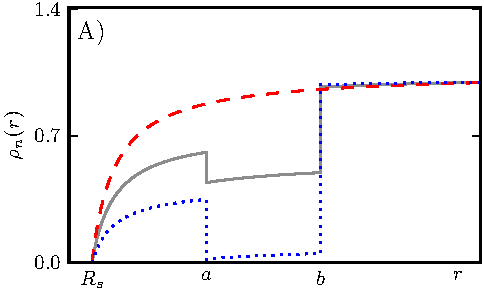
\includegraphics[width = 1 \textwidth]{plots/d1.pdf}
    \end{figure}
\end{minipage}
\begin{minipage}[t]{0.5 \textwidth}
    \begin{figure}[H]
        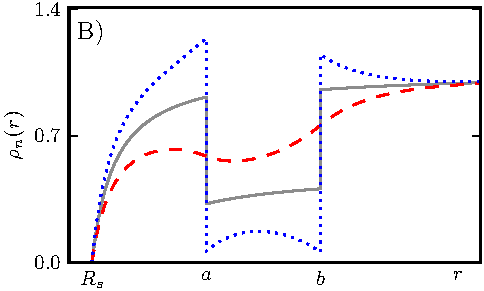
\includegraphics[width = 1 \textwidth]{plots/d2.pdf}
    \end{figure}
\end{minipage}
\begin{minipage}[t]{0.5 \textwidth}
    \begin{figure}[H]
        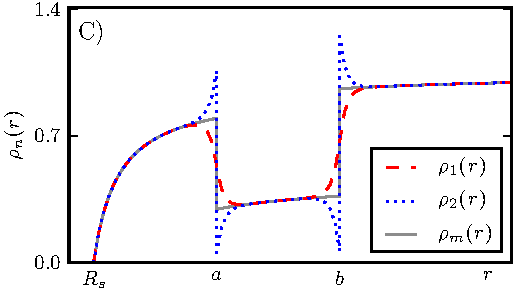
\includegraphics[width = 1 \textwidth]{plots/d3.pdf}
    \end{figure}
\end{minipage}\hspace{0.07\textwidth}\begin{minipage}[t]{0.43 \textwidth}
    \begin{figure}[H]
        \caption{Density profiles for repulsive fluctuating barrier. The densities of particles in state $m=1$ and state $m=2$ are depicted in dashed red, and dotted blue respectively. The decay length is given by A): $r_d = 250$, \newline B): $r_d=2.5$ and C): $r_d=0.25$. \label{rsd}}
    \end{figure}
\end{minipage}


\begin{minipage}[t]{0.5 \textwidth}
    \begin{figure}[H]
        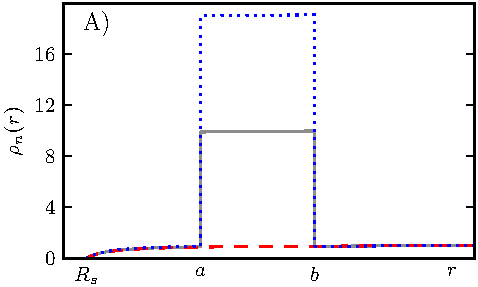
\includegraphics[width = 1 \textwidth]{plots/d4.pdf}
    \end{figure}
\end{minipage}
\begin{minipage}[t]{0.5 \textwidth}
    \begin{figure}[H]
        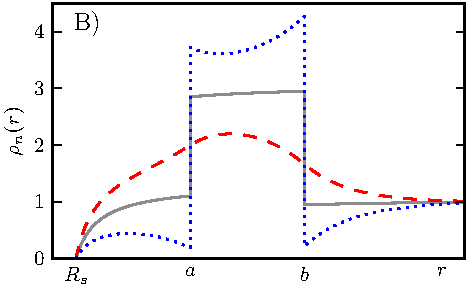
\includegraphics[width = 1 \textwidth]{plots/d5.pdf}
    \end{figure}
\end{minipage}
\begin{minipage}[t]{0.5 \textwidth}
    \begin{figure}[H]
        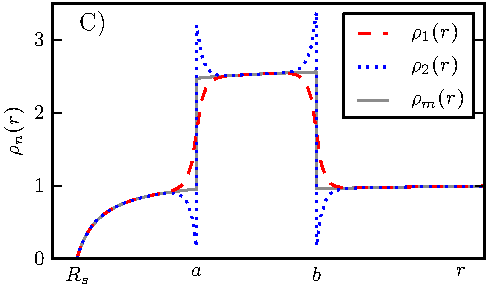
\includegraphics[width = 1 \textwidth]{plots/d6.pdf}
    \end{figure}
\end{minipage}\hspace{0.07\textwidth}\begin{minipage}[t]{0.43 \textwidth}
    \begin{figure}[H]
        \caption{Density profiles for attractive fluctuating barrier. The densities of particles in state $m=1$ and state $m=2$ are depicted in dashed red, and dotted blue respectively. The decay length is again given by A): $r_d = 250$, B): $r_d=2.5$ and C): $r_d=0.25$ \label{asd}}
    \end{figure}
\end{minipage} 
\newpage
\section{Flow Analysis}
\label{flow_analysis}
Density profiles only give information about where particles are. However, it is of interest how they got there and where they are going next. This is also necessary for the explanation of the behavior observed in part B) of figures \ref{rsd} and \ref{asd} in the previous section.
To investigate particle movement it is reasonable to use spatial and reactive fluxes for a further study of the system.
To do so the radial coordinate of the system is divided into different areas as depicted in figure \ref{fig:flowchart_scetch}.
\begin{figure}[H]
    \centering
    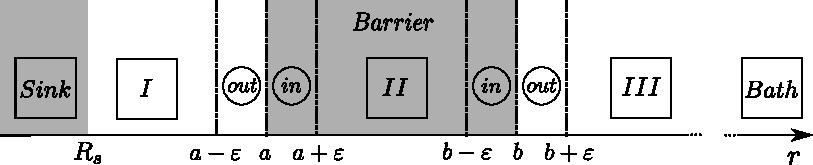
\includegraphics[width = .9 \textwidth]{plots/drawing.pdf}
    \caption{Sketch of the spatial discretization for the flow analysis of the system: The Sink and the Barrier are marked in gray. The circles represent narrow volumes of width $\varepsilon$ right at the barrier borders. $\varepsilon$ is set to be one tenth of the barrier width. The squares represent the remaining volumes between barrier and sink ($I$), between the barrier boundaries ($II$) and outside the sink ($III)$ . Each volume has the shape of a spherical shell (except the sink which is a sphere). Active and inactive particles are investigated separately in each of these volumes}
    \label{fig:flowchart_scetch}
\end{figure}
For each of these areas one examines the spatial fluxes from and to neighboring areas and the reactive fluxes from one particle state to the other. \\
For this purpose it is convenient to use the integral form of the continuity equation derived in \eqref{ce0}. To employ it in the actual problem one takes the density profiles to be constant in time such that its left hand side vanishes. Then the terms on the right hand side are calculated separately. The spatial fluxes at the volume boundaries:
\begin{equation}
    J_m^{(S)}(r_i) = \int_{r_i} \vec{j}_m(r) {\rm d} \vec{A}
    \label{spatial_flux}
\end{equation}
and the reactive fluxes from one particle species to the other:
\begin{equation}
    J_{mm'}^{(R)}(r_i,r_j) =\int_{r_i}^{r_j} \left\{ \mathbb{W}_{m'm}\rho_m - \mathbb{W}_{mm'} \rho_{m'} \right\} {\rm d} r
    \label{reaction_flux}
\end{equation}
where $r_i$ and $r_j$ are the radii $R_s$, $a-\varepsilon$, $a$ etc. of the spatial discretization given in figure \ref{fig:flowchart_scetch}.
These fluxes are then represented as arrows between the icons representing the corresponding areas as illustrated in figure \ref{fig:flowchart_scetch}. Active and inactive particles are depicted separately where the icons representing active particles are blue and the icons representing inactive particles are red. \\ \textbf{Interpreting the following flow diagrams it is important to note, that the flows depicted by the arrows are normalized to the largest value for each example. Therefore the arrows only represent \emph{relative importance of fluxes} and have no meaning for their absolute values!}
. \\ \vspace{-1.3 cm}

\begin{minipage}[t]{.372 \textwidth}
    \vspace{0.5 cm}
    \begin{figure}[H]
        \caption{Flow diagram for repulsive barrier: This plot shows spatial and reactive particle flows between different particle species (active particles are represented in blue, inactive particles are represented in red) and different spatial regions (see figure \ref{fig:flowchart_scetch} for reference) for the examples given in figure \ref{rsd}. The difference between the different plots is again the decay length which is equal to \newline A): $r_d=250$, B): $r_d=2.5$ and \newline C): $r_d = 0.25$.
    \label{fig:flow_repulsive}}
    \end{figure}
\end{minipage}\hspace{0.02 \textwidth}\begin{minipage}[t]{.608 \textwidth}
    \begin{figure}[H]
        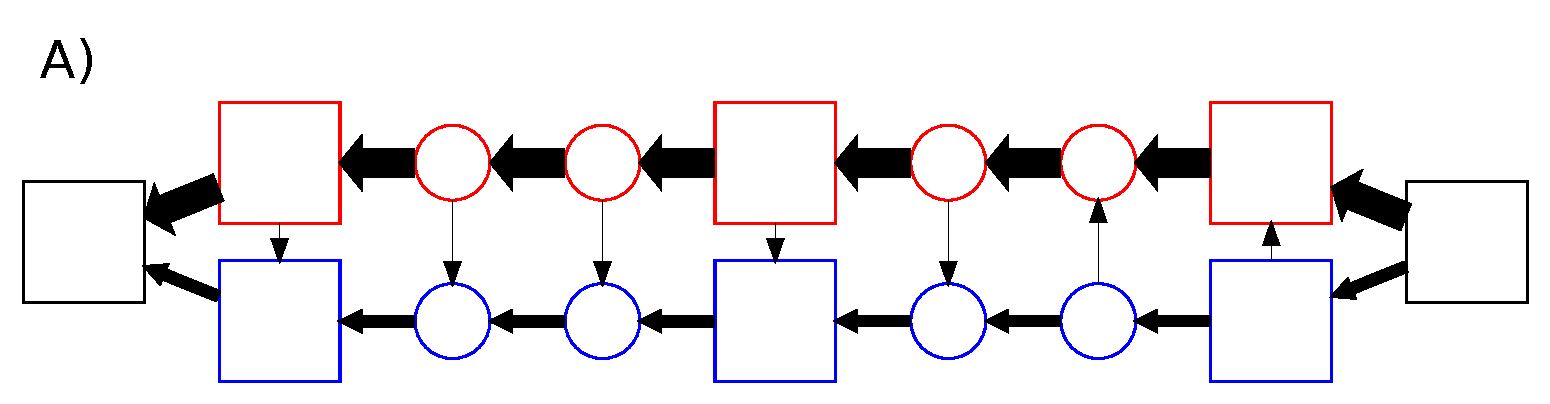
\includegraphics[width = 1 \textwidth]{plots/rep_flowchart0.pdf} 
        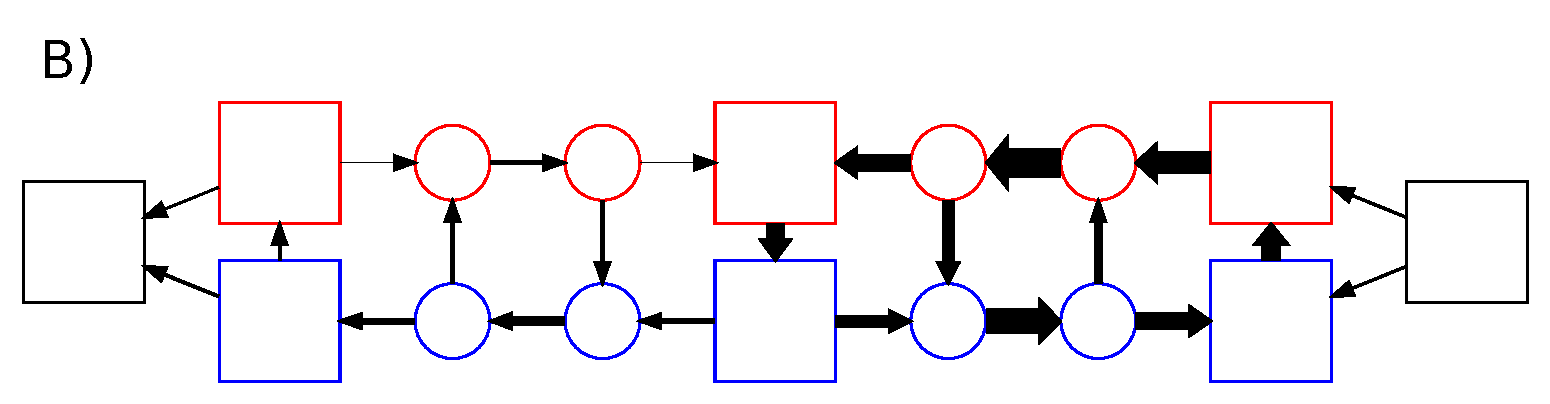
\includegraphics[width = 1 \textwidth]{plots/rep_flowchart1.pdf} 
        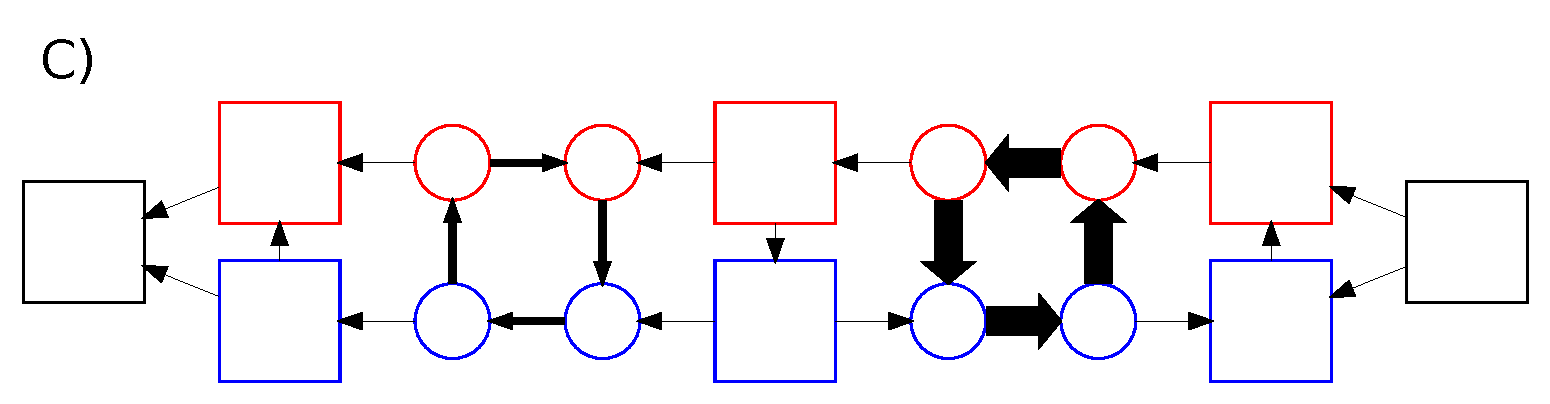
\includegraphics[width = 1 \textwidth]{plots/rep_flowchart2.pdf}
    \end{figure}
\end{minipage}
\vspace{0.5 cm} \\
It is obvious from this illustration that the system behaves qualitatively different depending on the decay length $r_d$.
\begin{itemize}
    \item For long decay length as in figure \ref{fig:flow_repulsive} A) it is visible from the very narrow arrows connecting red and blue icons that the particles in both states are independent in good approximation. Therefore inactive particles are not hindered by the barrier on their way from the bath to the sink whereas active particles have to overcome the potential barrier and are thus less likely to interact with the sink. Ether way, particles are very unlikely to change their state in the process. 
    \item For short decay length as in figure \ref{fig:flow_repulsive} C) the behavior is clearly different. Particle movement is closely tied to the potential boundaries at $r=a$ and $r=b$. There active particles are very likely to cross the boundary in downward direction only. Therefore the potential drives a spatial selection of particles that leads to an excess of active particles right outside and a deficit of active particles inside the barrier. The resulting difference in concentration of active and inactive particles at both sides of the barrier boundary leads to a strong reactive fluxes. Inside the barrier particles switch from inactive (red) to active (blue) and outside the barrier they switch from active to inactive state. The resulting imbalance of inactive particles draws them across the barrier from the out to the inside. As obvious from the flow diagram, the result is a strong \emph{circular current}. Since most of the particles switch states before they can diffuse more than $r_d$ away, the 
process is closely tied to the barrier boundaries. 
    \item For medium decay length as in figure \ref{fig:flow_repulsive} B) these circular currents are still existent but not so closely tied to the boundaries of the barrier. Therefore they overlap in space. This has the effect that once a particles has crossed the outer boundary of the barrier as part of one circular current it can switch to the other circular current to cross the inner boundary of the barrier. 
\end{itemize}
In the case of an attractive potential barrier the processes at work are quite similar. The differences to the repulsive case are outlined on the basis of the following flow diagrams: \vspace{-.5 cm} \\
\begin{minipage}[t]{.372 \textwidth}
    \vspace{.5 cm}
    \begin{figure}[H]
        \caption{Flow diagram for attractive barrier: This plot shows spatial and reactive particle flows between different particle species (active particles are represented in blue, inactive particles are represented in red) and different spatial regions (see figure \ref{fig:flowchart_scetch} for reference) for the examples given in figure \ref{asd}. The difference between the different plots is again the decay length which is equal to \newline A): $r_d=250$, B): $r_d=2.5$ and \newline C): $r_d = 0.25$.
    \label{fig:flow_attractive}}
    \end{figure}
\end{minipage}\hspace{0.02 \textwidth}\begin{minipage}[t]{.608 \textwidth}
    \begin{figure}[H]
        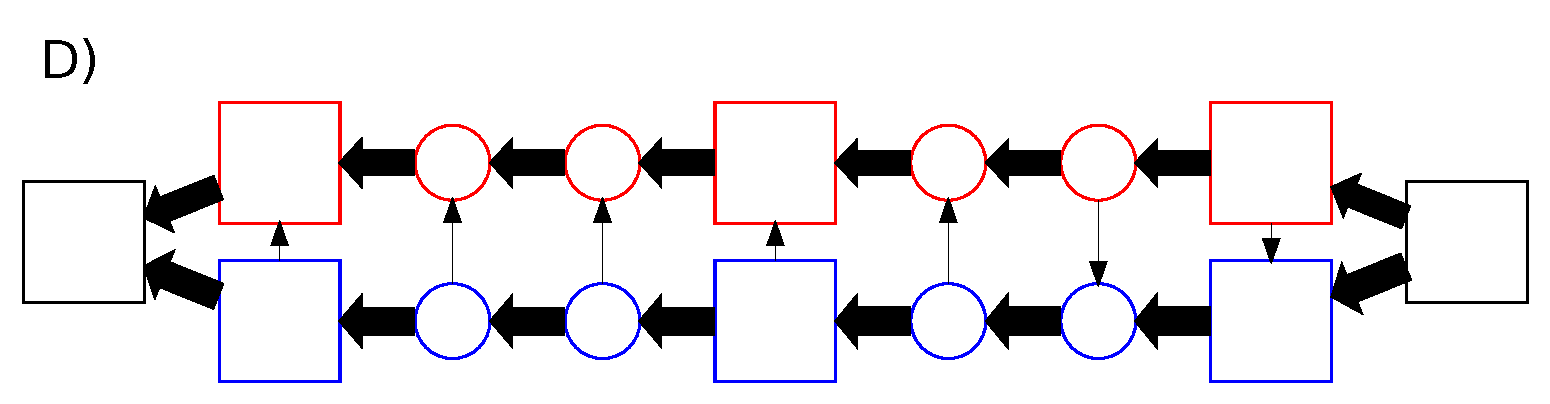
\includegraphics[width = 1 \textwidth]{plots/att_flowchart0.pdf}
        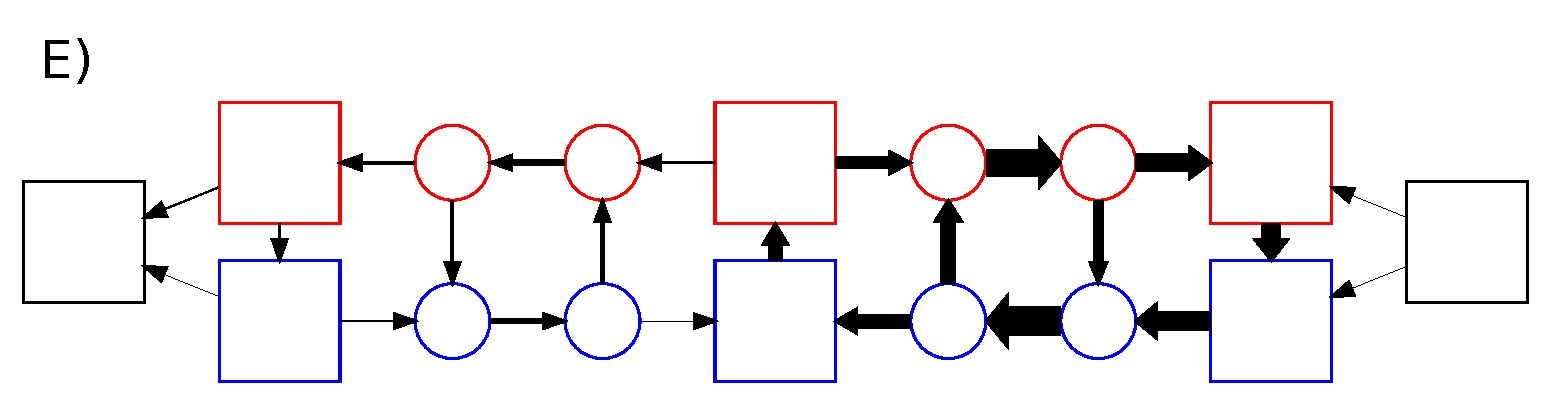
\includegraphics[width = 1 \textwidth]{plots/att_flowchart1.pdf}
        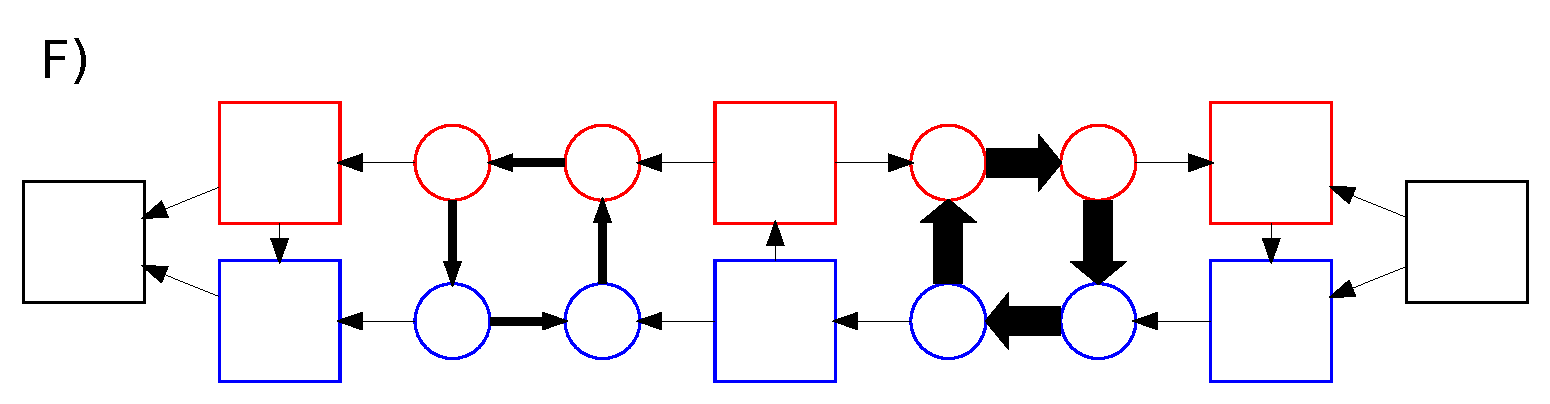
\includegraphics[width = 1 \textwidth]{plots/att_flowchart2.pdf}
    \end{figure}
\end{minipage}
\vspace{.5 cm} \\
The differences of these examples to the ones presented before in figure \ref{fig:flow_repulsive} can be pointed out one by one:
\begin{itemize}
    \item For long decay length as in figure \ref{fig:flow_attractive} D) the two particle species are independent from each other in good approximation. The difference to the former example is that the active particles are not hindered by the attractive barrier once the steady state is reached. They accumulate in the attractive potential until their concentration is high enough to to make it equally possible for particles to enter and leave the barrier (which is essentially given by the probability for particles to enter the potential). Therefore both particle species do equally contribute to the flux of particles from the bath to the sink.
    \item For short decay length as in figure \ref{fig:flow_attractive} F) the system again shows strong circular currents around the boundaries of the potential barrier. The difference is here that if active particles now cross the barrier in downward direction this means from the ``out'' to the ``in'' side. Therefore the circular currents are now directed in the other direction (clockwise vs. counter clockwise in this representation).
    \item For medium decay length as in figure \ref{fig:flow_attractive} E)  the two circular currents overlap just as they do in the case of a repulsive barrier. Therefore it is again likely for active particles to be drawn across the outer border of the potential by one current and then cross the boundary of the inner barrier as part of the other current.
\end{itemize}
This analysis has shown how the system behaves qualitatively different depending on the switching rate of the barrier $W$ or rather depending on the decay length $r_d$ of the particle densities. Knowing this, it is now time to turn to the key quantity in this investigation which is the reaction rate of particles interacting with the sink. 
\section{Absorption Rates}
Previously the focus was directed on the distribution of Brownian particles in the system. The distribution was explored for different magnitudes of the systems' decay length and qualitative differences were explained by the steady state flow of particles that emerged from the coupling of the barrier fluctuations to the diffusive particle movement.\\
The next section will explore the implications of these qualitative differences on the reaction rate of particles with the sink in the center of the system. This rate can be calculated from the density profiles via equation \eqref{Rate}. In the following the reaction rate is normalized to the Smoluchowski reaction rate $K_S$ \eqref{steady state ideal rate} for an ideal sink without any barrier . This way the influence of the potential barrier can be pointed out explicitly. \\
An analytic expression for the reaction rate is given in Appendix A.
Sadly, this form of the solution is longish, bulky and does not tell very much about the actual behavior of the reaction rate. Nevertheless, it can be used to plot the reaction rate in the case of the two examples that were studied so far: \\
\begin{minipage}[t]{0.5 \textwidth}
    \begin{figure}[H]
        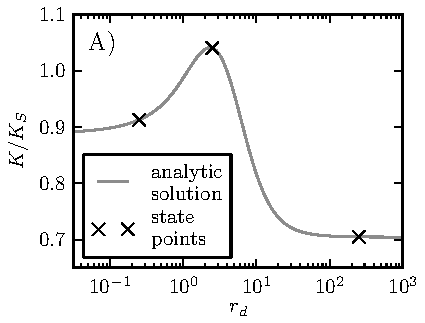
\includegraphics[width = 1 \textwidth]{plots/rb_rate.pdf}
    \end{figure}
\end{minipage}\begin{minipage}[t]{0.5 \textwidth}
    \begin{figure}[H]
        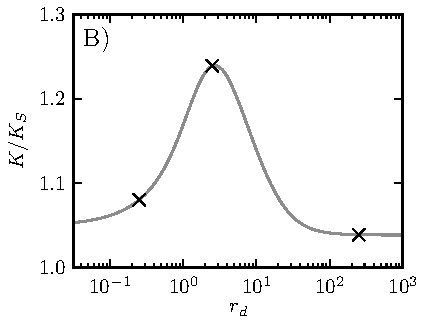
\includegraphics[width = 1 \textwidth]{plots/ab_rate.pdf}
    \end{figure}
\end{minipage}

\begin{minipage}[t]{1 \textwidth}
    \begin{figure}[H]
        \caption{Reaction rate of Brownian particles depending on the decay length of particle density for A) a repulsive barrier and B) an attractive barrier. The decay length and resulting reaction rate for the examples illustrated before are marked with black crosses. Those from figures \ref{rsd} and \ref{fig:flow_repulsive}  are marked in A), and those from figures \ref{asd} and \ref{fig:flow_attractive} are marked in B).\label{reaction_rate_examples}}
    \end{figure}
\end{minipage}
\vspace{.5 cm} \\
It is obvious from these plots that the reaction rate converges to finite values for very small and very large decay length and that it takes some maximum value in between. \\
Similar behavior has been studied for escape rates of Brownian particles trapped in fluctuating potentials. In this case the mean first passage time of the trapped particle over the barrier depends on the properties of the potential fluctuations. This has been extensively studied for different barrier shapes and different types of fluctuations \cite{Doering1992, Zurcher1993, Hanggi1994, Pechukas1994,Reimann1995a, Reimann1995}. \\
When Charles Doering and Jonathan Gouda first observed the phenomenon in 1992 \cite{Doering1992} they studied a particle that was trapped between a reflecting wall and a piecewise linear potential barrier that was subject to dichotomous Markovian noise. They observed that the mean first passage time of the particle over the barrier converged to finite values for very small and very long correlation times of the barrier fluctuations and exhibits a minimum in between. For this behavior they coined the term\textbf{ \emph{resonant activation}}.\\
Although this has only been studied for escape problems so far, the results presented here strongly suggest that it is also valid to use the term in the case of reaction rates over fluctuating barriers. \par
Even the underlying processes that have been studied in the previous section can be identified with those, that were found to be responsible for resonant activation in escape problems.
Referring to a first review paper on the topic published by Peter Reimann and Peter H\"anggi in 1997 \cite{Reimann1997} the case of a repulsive barrier can be identified with what they call ``Type I'' potentials, where particles enter the barrier region when it is in a low state and then get lifted up when the barrier switches to be subsequently able to escape. The case of an attractive barrier can be identified with what they call ``Type II'' or breathing barrier. In this case the part of the barrier that actually fluctuates is located right before the actual boundary that has to be overcome. The particle can enter the fluctuating area while it is in a low state, be then lifted when it changes to a high state and be subsequently able to cross the actual boundary. \par

Now, the next step in studying the vast expression that was derived for the reaction rate \eqref{two_state_rate} is evaluating some limits and trying to make sense of them in a physical way.
\section{Slow Fluctuation Limit}
\label{lim_long_rd}
For slow fluctuations of the potential barrier the decay length $r_d$ and therefore the spatial influence of the potential barrier becomes large compared to the length scale of the system. \\ 
To evaluate this limit, one uses equation \eqref{two_state_fpe} with symmetric rates, takes the limit of $W \rightarrow 0$ and considers the steady state case.
This results in two independent equations for the two particle species:
\begin{align}
    \frac{\partial \rho_1(r,t)}{\partial t} &= \vec \nabla \left[ D \vec \nabla \rho_1(r,t) \right], \\ \nonumber
    \frac{\partial \rho_2(r,t)}{\partial t} &= \vec \nabla \left[\rho_2(r,t) \vec \nabla \frac{U_2(r)}{\gamma} + D \vec \nabla \rho_2(r,t) \right]
    \label{two_state_fpe_W_to_0}
\end{align}
where $U_2$ has the form given in \eqref{step_potential}. \\
It is assumed that the detailed balance assumption and therefore the boundary condition for $r \rightarrow \infty$ remains valid despite the formal independence of the particle species.\\
The reaction rates for these independent equations can be calculated using the expressions given in \eqref{steady state ideal rate} and \eqref{K_Debye}. The combined rate can be derived as the weighted average of the two independent rates. Since the transition rates are taken to be symmetric, this results in:
\begin{align}
    K &= \frac{1}{2} \left[ 4 \pi D R_s^2 + 4 \pi D  \left\{\int_{R_s}^{\infty} \frac{\exp \left[ \frac{U_2(r')}{K_B T}\right]}{r'^2} \rm d r' \right\}^{-1} \right] \\ \nonumber
    &= 2 \pi D \left[ R_s^2 +\left\{\int_{R_s}^{a} \frac{1}{r'^2} \rm d r' + \int_{a}^{b} \frac{\exp \left[ \frac{U_2(r')}{K_B T}\right]}{r'^2} \rm d r' + \int_{b}^{\infty} \frac{1}{r'^2} \rm d r' \right\}^{-1} \right].
\end{align}
One evaluates the integrals, divides by the Smoluchowski reaction rate $K_S = 4 \pi D$, sets $R_s$ to one and substitutes $U_2/K_B T$ by $u$ to get:
\begin{align}
    \frac{K}{K_{S}} &= \frac{1}{2} \left[1 + \left\{ 1 -\frac{1}{a} + e^u \left(\frac{1}{a} - \frac{1}{b}  \right) + \frac{1}{b} \right\}^{-1} \right] \nonumber \\
    &= \frac{1}{2}\left[ 1 + \left\{ 1 + \left( \frac{1}{a} - \frac{1}{b} \right)\left( e^u -1 \right) \right\}^{-1} \right] \nonumber \\
    &= \frac{1}{2} \left[ 1 + \left\{ 1 - \frac{(b - a)}{ab}\left(1 - e^u \right) \right\}^{-1} \right] \nonumber \\
    &= \frac{1}{2} \left[ 1 + \frac{ab}{ab - \left( b-a \right)\left(1 - e^u \right)} \right].
    \label{two_state_K_slow}
\end{align}
The result of this somewhat intuitive calculation can then be compared to the slow switching limit of equation \eqref{two_state_rate}.
It proves to be sufficient to do a Taylor expansion around $\alpha_0 = 0$ to obtain
\begin{equation}
    \frac{K}{K_{S}} \approx \frac{(b-a)(1-e^u)-2ab }{2 \left((b-a) \left(1-e^u\right)-ab\right)} + \frac{  (b-a)^2\left(1-e^u\right)^2}{4 \left(ab + (b-a)(1-e^u)\right)^2} \alpha.
    \label{ksa}
\end{equation}
Where the leading term can be modified to take the form
\begin{equation}
    \lim_{\alpha \rightarrow 0} \frac{K}{K_{S}} =\frac{1}{2}\left(1+ \frac{ab}{ab-(b-a) \left(1-e^u\right)}\right).
    \label{klim0a}
\end{equation}
This is exactly the result, that was obtained in the previous calculation.
\section{Fast Fluctuation Limit}
\label{lim_short_rd}
For fast fluctuations of the potential barrier, there is another way to deal with equation \eqref{two_state_fpe}. In the limit of $W \rightarrow \infty$ the diffusion term can be neglected compared to the reactive terms, such that in the case of symmetric rates $\rho_1(r) \equiv \rho_2(r) = 2\rho(r)$ holds for all $r>R_s$. Therefore both equations can be added resulting in: 
\begin{equation}
    2 \frac{\partial \rho(r,t)}{\partial t} = \vec \nabla \left[\rho(r,t) \vec \nabla \frac{U_2(r)}{\gamma} + 2 D \vec \nabla \rho(r,t) \right].
    \label{fast_limit_fpe}
\end{equation} 
In other words this means that the timescale of the switching of particles between different states is much smaller than the timescale of spatial movement of the particles. As a result all particles move subject to a constant potential of mean force that is calculated as the weighted average of the potential in its different states. \\
Also, in the steady state case the time derivative of the density vanishes:
\begin{equation}
    0 = \vec \nabla \left[\rho(r,t) \vec \nabla \frac{U_2(r)}{2\gamma} + D \vec \nabla \rho(r,t) \right]
\end{equation}
such that the steady state rate can be calculated using the Debye formula \eqref{K_Debye}:
\begin{align}
    K &=  4 \pi D \left\{\int_{R_s}^{\infty} \frac{\exp \left[ \frac{U_2(r')}{2 K_B T}\right]}{r'^2} \rm d r' \right\}^{-1} \nonumber \\
    &= 4 \pi D \left\{\int_{R_s}^{a} \frac{1}{r'^2} \rm d r' + \int_{a}^{b} \frac{\exp \left[ \frac{U_2(r')}{2K_B T}\right]}{r'^2} \rm d r' + \int_{b}^{\infty} \frac{1}{r'^2} \rm d r' \right\}^{-1}.
    \label{mean_potential_rate}
\end{align}
The evaluation of the integrals, substitution of $U_2/K_B T$ with $u$ and the normalization by the Smoluchowski reaction rate $K_S$ from equation \eqref{steady state ideal rate} results in:
\begin{equation}
    \lim_{\alpha \rightarrow \infty} \frac{K}{K_S} = \frac{ab}{ab - (b-a)(1-e^{u/2})}.
    \label{K_fast_limit_1}
\end{equation}
A useful examination of the fast switching limit of equation \eqref{two_state_rate} requires a bit more work.
To find the behavior in the limit of $r_d \ll 1 $, i.e. $\alpha \gg 1$ one takes a closer look at the different exponents that occur in the numerator and denominator of equation \eqref{two_state_rate}. Namely:
\begin{align}
& e_1 = (3a+b)\alpha, \nonumber \\
& e_2 = (2+2b)\alpha, \nonumber \\
& e_3 = (2+a+b)\alpha, \nonumber \\
& e_4 = 4a\alpha, \nonumber \\
& e_5 = (2+2b)\alpha \quad \textrm{and} \nonumber \\
& e_6 = (2a+2b)\alpha.
\end{align}
Using the fact that $b > a > 1$ one finds that for $\alpha \gg 1$ the terms containing $e_6$ dominate all others. Therefore numerator and denominator can be reduced to
\begin{align*}
    F_1' =& ( 1 + a \alpha + e^u (-1 + 3 a \alpha)) (-1 + 3 b \alpha + e^u (1 + b \alpha))\\
    F_2' =& (-1 + (4 - 3 a + b) \alpha + (2 a - 2 b + 3 a b) \alpha^2 + e^{2 u} (-1 + (4 + a - 3 b) \alpha \\
          &+ 3 (a (-2 + b) + 2 b) \alpha^2) + 2 e^u (1 + (-4 + a + b) \alpha + (2 a - 2 b + 5 a b) \alpha^2)).
\end{align*}
If then only linear and quadratic terms in $\alpha$ are collected one receives an expression that turns out to be a reasonably good approximation of the fast switching behavior of the solution: 
\begin{align}
    \frac{K}{K_{S}} \approx &a \left(3 e^u+1\right) \left(e^u (b x+1)+3 b x-1\right)-b \left(2 e^u+e^{2 u}-3\right) / \nonumber \\
                          &\left\{a \left(e^{2 u} (3 (b-2) x+1)+2 e^u ((5 b+2) x+1)+3 b x+2 x-3\right) \right.  \nonumber \\
                          & \left. +\left(e^u-1\right) \left(b \left(3 e^u+1\right) (2 x-1)+4 \left(e^u-1\right)\right) \right\}
    \label{kla}
\end{align}
and in the actual limit of $\alpha \rightarrow \infty$ one obtains: 
\begin{equation}
    \lim_{\alpha \rightarrow \infty} \frac{K}{K_{S}} = \frac{a b \left(e^u+3\right)}{ab \left(e^u+3\right)-2(b-a)(1-e^u)}.
    \label{kliminfa}
\end{equation}
This can be simplified to 
\begin{align}
    \lim_{\alpha \rightarrow \infty} \frac{K}{K_S} &= \frac{ab}{ab - (b-a)(1-e^{u/2}) \kappa}, \\
    \kappa &= \frac{2(1+e^{u/2})}{e^u + 3}.
    \label{K_fast_limit_2}
\end{align}
This is clearly not equal to the limit that was obtained in equation \eqref{K_fast_limit_1}.\par
Now, lets see, if it is possible to understand this difference and to learn something from it. To do so it is useful to properly outline the differences in the derivation of these results.
Therefore it is crucial to realize that it is in fact \emph{two} limits that were taken in the process and that their order differed between the two calculations. One limit is that of the decay length $r_d \rightarrow 0$. The other limit concerns the spatial area of the change of the potential barrier, i.e. the width $r_F$ of the spherical shell in which the Brownian particles are actually subject to a force from the barrier. \\
\vspace{-.8 cm} \\
\begin{minipage}[t]{0.372 \textwidth}
    \begin{figure}[H]
        \caption{Simple sketch to point out the order of limits taken for the derivation of equation \eqref{K_fast_limit_1} and \eqref{K_fast_limit_2}. Both derivations uncouple the original equations to derive an expression for the fast switching limit of the reaction rate but the order of limits differs. \label{sketch_of_limits}}
    \end{figure}
\end{minipage}\hspace{0.01 \textwidth} \begin{minipage}[t]{.608 \textwidth}
\begin{figure}[H]
    \centering
    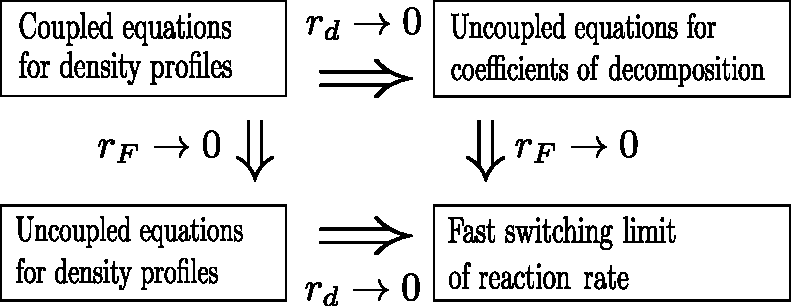
\includegraphics[width = 1 \textwidth]{plots/limits.pdf}
\end{figure}
\end{minipage}\par
Like it is illustrated in figure \ref{sketch_of_limits} the difference is the following: For the derivation of \eqref{K_fast_limit_1} the \emph{first} limit was that of $r_d \rightarrow 0$ and the \emph{second} limit was that of $r_F \rightarrow 0$ whereas for the derivation of \eqref{K_fast_limit_2} the \emph{first} limit was that of $r_F \rightarrow 0$ and the \emph{second} was that of $r_d \rightarrow 0$. \\
Since in general it is not equivalent to take limits in exchanged order it is not unexpected that the resulting expressions differ. The question is now: What does this mean in physical terms? \\

\newpage
\section{Numeric Study of Smooth Potential Barriers}
\label{Numeric_Study}
The easiest way to get an insight into the final question posed in the last section is to take a closer look at what actually happens, if the potential barrier does not vary in sharp jumps but does so on a finite length scale.
Therefore one examines how the reaction rate depends on the decay length of the particle density given a fixed but finite area on which the barrier changes. The natural way to do this is the application of a potential barrier that resembles a step function in shape and has a parameter to tweak this similarity. A generalized Gaussian:
\begin{equation}
    U_2(r) = U_2 \cdot \exp \left[ - \left( \frac{r_0 - r}{d} \right)^{2n} \right]
    \label{generalized_gaussian}
\end{equation}
with $r_0-d=a$ and $r_0+d=b$ serves this purpose well. The parameter $n$ can be used to control the width $r_F$ of the area of changes in the potential. It decreases as $n$ increases. \\
To compare the analytic results with numeric simulations they have to be derived with the same boundary conditions. Since it is not possible to set boundary conditions at infinity in numeric simulations one has to modify the boundary conditions \eqref{bcinf} in the analytic calculations. This can be done by setting 
\begin{equation}
    \vect{\rho}(R_m) = \vect{\rho}^{(eq)}
    \label{BC_for_numerics}
\end{equation}
where $R_m$ is the radius of the simulation domain. The numeric results for the reaction rate were derived by integrating the equations for the composite Markov process \eqref{two_state_fpe} using the method of lines described in section \ref{method_of_lines}. The results of this procedure are presented in the figure \ref{numeric}: \vspace{-0.5 cm}\\

The behavior that is observed in the comparison of numeric results with the analytic solution for the fluctuating step potential (FSP) \eqref{two_state_rate} and the rate over the static potential of mean force (PMF) \eqref{K_fast_limit_1} tells a couple of interesting things:
\begin{itemize}
    \item First, the resonant activation phenomenon that is observed for step potentials does also emerge for smooth potentials and is not an artefact or a mathematic curiosity. In fact the effect does get even stronger if the change of the potential happens on a finite length scale.
    \item Second, for $r_d \gg r_F$ the numeric results are well represented by the solution derived in \ref{Reaction_Rates_over_Fluctuating_Barriers} whereas for $r_d \ll r_F$ they show good agreement with the rate over a PMF. It is especially interesting, to have a closer look at the transition from the first to the latter case.
\end{itemize}
\begin{minipage}[t]{.5 \textwidth}
    \begin{figure}[H]
        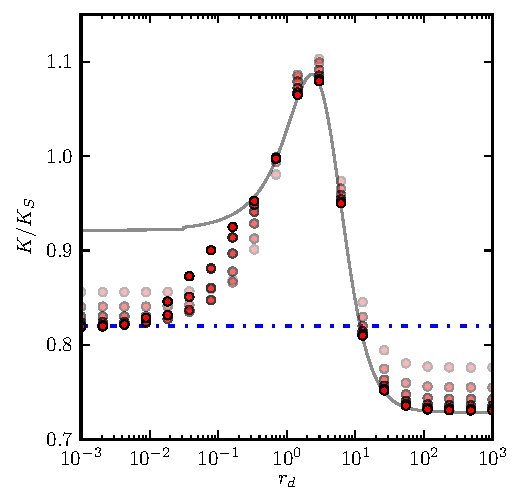
\includegraphics[width = 1 \textwidth]{plots/rb_cs.pdf}
    \end{figure}
\end{minipage}\begin{minipage}[t]{.5 \textwidth}
    \begin{figure}[H]
        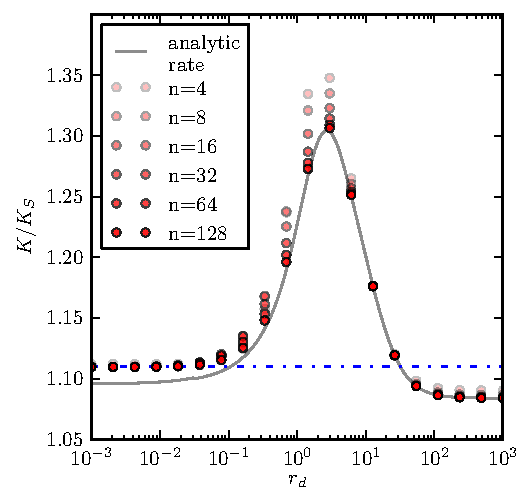
\includegraphics[width = 1 \textwidth]{plots/ab_cs.pdf}
    \end{figure}
\end{minipage}

\begin{minipage}[t]{1 \textwidth}
    \begin{figure}[H]
        \caption{Comparison of numeric and analytic results for repulsive (\emph{left}) and attractive (\emph{right}) fluctuating barrier. The numeric results are obtained via the method of lines \ref{method_of_lines}. The reaction rate over the potential of mean force \eqref{K_fast_limit_1} is indicated by the dashed blue line. The analytic solution over the fluctuating step shaped barrier in equation \eqref{two_state_rate} is indicated by a solid grey line. The radius of the simulation domain is $R_m=30 R_s$. The other parameters are the same as in the previous examples and given in \ref{Parameters}. The analytic solution represents the numeric results very well for large $r_d$ and small $r_F$. The numeric results converge away from the analytic solution for the step shaped fluctuating barrier and towards the rate over the potential of mean force for small $r_d$. Note that the smaller $r_F$ (large $n$) of the potential, the smaller the $r_d$ at which the transition takes place.\label{numeric}}
    \end{figure}
\end{minipage} \vspace{0.5 cm} \\

As it can be seen especially for the case of the repulsive barrier, the transition of numeric results from the description by a FSP to a PMF takes place at a different decay length for different spatial extend of the changes of the potential barrier.  The smaller the spatial extent of the changes $r_F$, the smaller the decay length $r_d$ at which the transition takes place. \\
One possible explanation for this can be given in terms of particle fluxes: In the case of the FSP one has $r_F=0$ and therefore the total reactive flux in the region of potential change vanishes. In the case of the PMF it is assumed that the reactive fluxes are strong enough to make both particle species have the same spatial distribution. In other words: In the case of a FSP the area of potential change is dominated by spatial fluxes whereas in the case of a PMF it is dominated by reactive fluxes.\\
Another possible explanation can be given in terms of times: In the case of the FSP the decay time $\tau_R = W/2$ of the state of a particle is much larger than the time $\tau_S$ that it takes for a particle to cross the area of potential change (since the area is actually of zero spatial extent). In the case of the PMF it is the other way around (since the inverse of the switching rate goes to zero). For a derivation of the decay time $\tau$ please refer to Appendix A.\\
The neat thing about these two ways of explaining the situation is that they are essentially the same and that they both give  an estimate for the parameter range in which eater the FSP or the PMF description is valid, and consequently where the transition from one to the other takes place.
For the PMF [FSP] the reactive flux and the spatial flux driven by the potential $J^{(R)}$ and $J^{(F)}$ in the region of potential change fulfill the following relation:
\begin{equation}
    J^{(F)} \ll[\gg] J^{(R)}.
\end{equation}
If the change of the potential is assumed to take place at a radius $r_0$ the according sphere surface $A$ and the volume of the potential change $V$ can be assumed to be roughly $A=4 \pi r_0^2$ and $V=4 \pi r_0^2\cdot r_F$. With this the previous expression reads:
\begin{equation}
    \frac{\rho(r_0)}{\gamma}\frac{{\rm d}U(r_0)}{{\rm d}r} A \ll[\gg]\rho(r_0) W V.
\end{equation}
    Since in the overdamped limit the mean velocity of a particle is given by $\bar{v}(r) = f(r)/\gamma$ this can be written as:
\begin{align}
    \frac{\bar{v}}{r_F} & \ll[\gg] W \nonumber \\
    \frac{1}{\tau_S} & \ll[\gg] \frac{2}{\tau_R}.
\end{align}
Which is the equivalence of the flux and the traveling resp. reaction time argument that was to be shown.
Both arguments give an estimation to when one or the other description is a valid approximation to calculate the reaction rate:
\begin{equation}
    \frac{\Delta U}{K_B T} \ll[\gg] \frac{r_F}{2 r_d}
    \label{val_estimate}
\end{equation}
This last result gives the parameter ranges in which the FSP [PMF] description is valid and shows that the decay length at which the transition between both descriptions takes place is defined by the hight of the potential barrier and the width of the area of its boundary.
\section{Summary}
In the previous section a simple example of reaction rates over a fluctuating barrier revealed some interesting effects. It turned out that resonant activation as previously seen with escape problems does also appear in reaction rates over fluctuating barriers. The effect was explained by an analysis of spatial and reactive particle fluxes and validated by numeric results. At the analysis of the fast switching limit it became obvious that the solution for the fluctuating step potential does inherently not reproduce the natural result of an effective potential of mean force. As a result of the analysis of this ambiguity an estimate for the validity of both descriptions was derived.

\newpage
\section{Influence of Barrier Spacing}
Until now, the boundaries of the potential barrier were fixed to $a=6 R_s$ and $b=11R_s$ and the main focus was directed on the influence of the decay length $r_d$. Since this is understood quite well now, the next section will have a closer look on the impact of the barrier spacing.\\
The barrier spacing is reasonably described by two free parameters. First, the ratio of the gap between barrier and the sink and the width of the barrier $g$ and second, its overall length scale $l$ relative to the radius of the Sink $R_s$:
\begin{equation}
    \frac{a}{R_s} - 1 = l, \qquad \frac{b-a}{R_s} = g \cdot l
    \label{spacing_variables}
\end{equation}
With these the relative and the overall spacing of the barrier can be varied independently. 
It would be interesting to know how these parameters influence the decay length that maximizes the reaction rate. Unfortunately the expression for the reaction rate \eqref{two_state_rate} is such, that its discussion leads to transcendental equations that can not be solved analytically. Therefore the influence of the barrier spacing and the barrier gap to width ratio can only be investigated qualitatively and numerically. Next the influence of the barrier gap to width ratio $g$ will be examined first. \\

\begin{minipage}[t]{.5 \textwidth}
    \begin{figure}[H]
        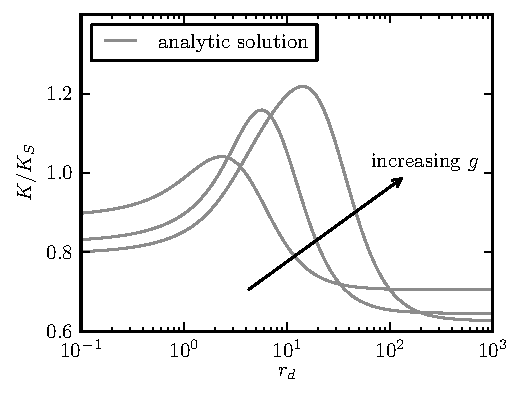
\includegraphics[width = 1 \textwidth]{plots/g2_rb_rates.pdf}
    \end{figure}
\end{minipage}\begin{minipage}[t]{.5 \textwidth}
    \begin{figure}[H]
        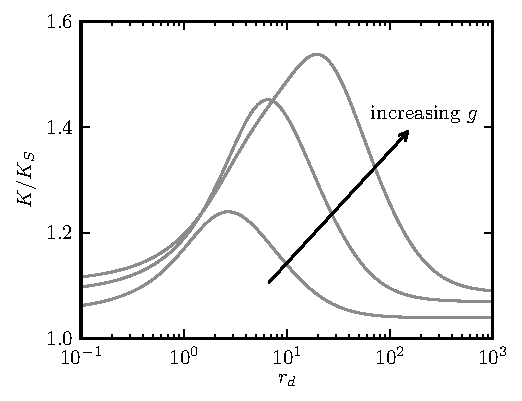
\includegraphics[width = 1 \textwidth]{plots/g2_ab_rates.pdf}
    \end{figure}
\end{minipage}

\begin{minipage}[t]{1 \textwidth}
    \begin{figure}[H]
        \caption{Reaction rates for different barrier gap to width ratio $g = 1, 4 ,16$ for repulsive fluctuating barrier (\emph{left}) and attractive (\emph{right}) fluctuating barrier. The overall barrier length scale $l$ is equal to $l=1 R_s$. The other parameters are given in \ref{Parameters}. It is obvious that the resonant activation effect also becomes more pronounced as the relative barrier width increases.\label{fig:var_g}}
    \end{figure}
\end{minipage} \vspace{0.5 cm} \\

The plots in figure \ref{fig:var_g} show, that influence of the barrier gap to width ratio $g$ is qualitatively different than that of the overall barrier spacing $l$. In the case of a repulsive barrier the reaction rates in the long and short decay length limits decrease if $g$ increases where it increased when $l$ increased. In the case of an attractive barrier the reaction rate in the long and short decay length limits increase if $g$ increases where it decreased when $l$ increased.
In both cases an increase in the gap to width ratio $g$ increases the decay length that maximizes the reaction rate and the resulting maximum reaction rate. Especially in the case of an attractive barrier it is obvious that the range of decay lengths that significantly increase the reaction rate becomes wider if $g$ increases. \\

The impact of the overall barrier spacing $l$ on the reaction rate is studied next.

\vspace{-0.5 cm}
\begin{minipage}[t]{.5 \textwidth}
    \begin{figure}[H]
        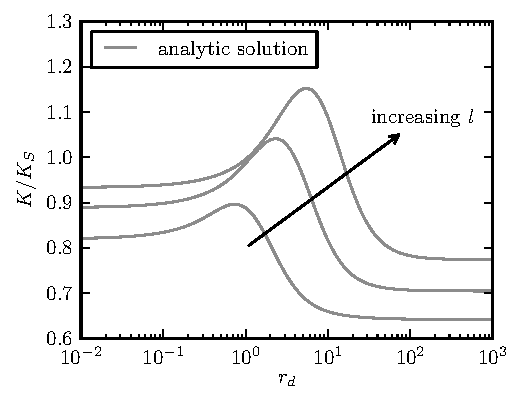
\includegraphics[width = 1 \textwidth]{plots/l2_rb_rates.pdf}
    \end{figure}
\end{minipage}\begin{minipage}[t]{.5 \textwidth}
    \begin{figure}[H]
        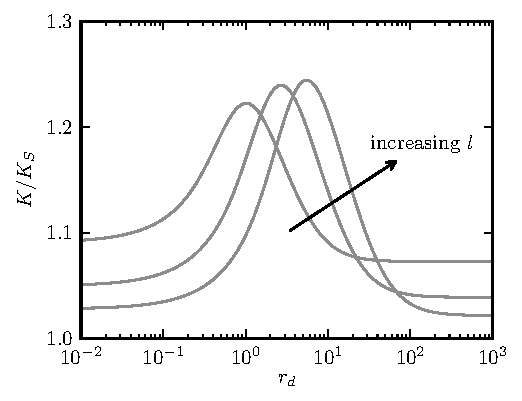
\includegraphics[width = 1 \textwidth]{plots/l2_ab_rates.pdf}
    \end{figure}
\end{minipage}\\
\begin{minipage}[t]{1 \textwidth}
    \begin{figure}[H]
        \caption{Reaction rates for different barrier spacing $l = 2 R_s, 5 R_s ,10 R_s$ for repulsive fluctuating barrier (\emph{left}) and attractive fluctuating barrier (\emph{right}). The ratio of the barrier width and the gap between sink and barrier $g$ is equal to one. The other parameters are given in table \ref{Parameters}. It is obvious that the resonant activation effect becomes more pronounced as the barrier spacing increases.\label{fig:var_l}}
    \end{figure}
\end{minipage} \vspace{0.5 cm} \\
The plots in figure \ref{fig:var_l} show that the barrier spacing has different impact on the long and short decay length limits of the reaction rate for in case of an attractive or repulsive barrier.
In the case of a repulsive barrier a larger barrier spacing increases the reaction rate in the short and long decay length limits. In the case of an attractive barrier a larger barrier spacing decreases the reaction rate in the short in long decay length limits. In both cases the decay length that maximizes the reaction rate as well as the resulting maximum reaction rate increase with a larger barrier spacing. The increase in the maximum reaction rate is stronger when the barrier is repulsive.\\
Further investigation of the dependence of the maximum reaction rate on the barrier spacing can be done numerically. Therefore one evaluates the roots of the first derivative of the analytic expression of the reaction rate given in equation \eqref{two_state_rate}. \\
\vspace{-0.5 cm}
\begin{minipage}[t]{.5 \textwidth}
    \begin{figure}[H]
        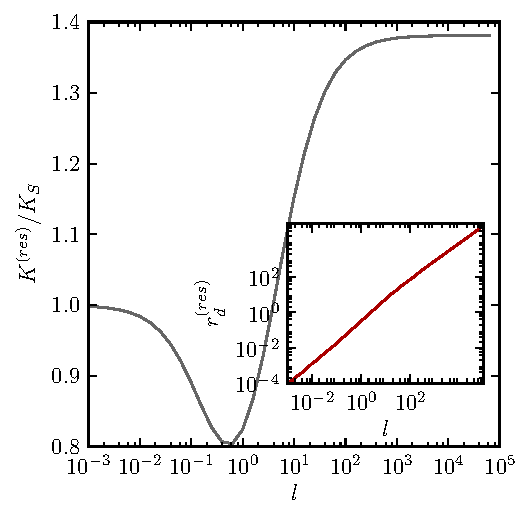
\includegraphics[width = 1 \textwidth]{plots/rep_l.pdf}
    \end{figure}
\end{minipage}\begin{minipage}[t]{.5 \textwidth}
    \begin{figure}[H]
        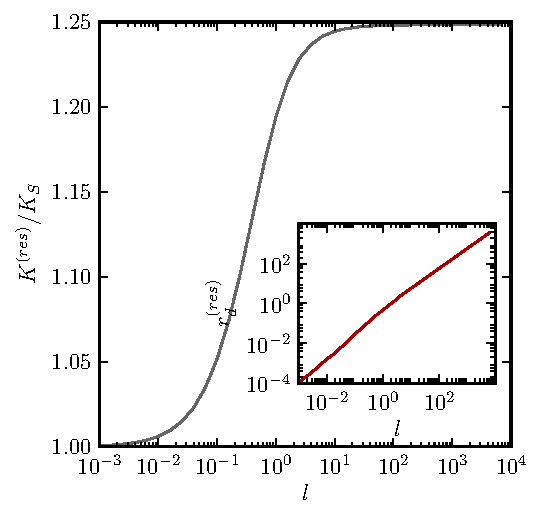
\includegraphics[width = 1 \textwidth]{plots/att_l.pdf}
    \end{figure}
\end{minipage}\\
\begin{minipage}[t]{1 \textwidth}
    \begin{figure}[H]
        \caption{Numeric evaluation of the maximum reaction rate $K^{(res)}$ depending on barrier spacing $l$ for repulsive fluctuating barrier (\emph{left}) and attractive fluctuating barrier (\emph{right}). The subplot gives the decay length $r^{(res)}$ that maximizes the reaction rate for each given barrier spacing $l$. The ratio of the barrier width and the gap between sink and barrier $g$ is equal to one. The other parameters are given in table \ref{Parameters}. It is obvious that the maximum reaction rate saturates for very large barrier spacing and that it becomes equal to the Smoluchowski reaction rate $K_S$ for a sink without barrier for very small barrier spacing. \label{fig:res_l}}
    \end{figure}
\end{minipage} \vspace{0.5 cm} \\

It is obvious from the plots in figure \ref{fig:res_l} that the maximum reaction rate for both, the attractive and the repulsive fluctuating barrier converge to the Smoluchowski reaction rate \eqref{steady state ideal rate} if the barrier spacing $l$ goes to zero. For very large barrier spacing the reaction rate converges to a finite value in both cases. \\
For the attractive fluctuating barrier the maximum reaction rate interpolates monotonously between these two values. For the repulsive fluctuating barrier the reaction rate has a local minimum. A possible explanation for this is, that for very small $l$ the barrier has no influence at all (this is in fact the case for barriers of finite hight, as will be shown in the following sections). For small but finite barrier spacing the barrier is mainly hindering particles from crossing and contacting the sink and only for larger barrier spacing the effect of overlaying circular currents illustrated in figure \ref{fig:flow_repulsive} of section \ref{flow_analysis} becomes stronger than the inherent shielding effect of the barrier.\\
Note that for large $l$ this can lead to reaction rates that are significantly (up to 40 \%) higher than than the reaction rate without a barrier and also higher than the highest possible reaction rate over a fluctuating attractive barrier.\\
So if this effect can be found in experiments where one usually only observes time averaged parameters such as the potential of mean force of the barrier and the reaction rate this must look confusing. The rate over the repulsive potential is notably higher than the rate over the attractive potential although classical Debye rate theory as outlined in \ref{The_Debye_Reaction_Rate} suggests the opposite.

\section{Influence of the Barrier Height}
This section investigates the influence of the barrier hight on the reaction rate. It gives the limiting behavior of the system for an infinitely attractive and an infinitely repulsive barrier and outlines the behavior for intermediate barrier heights.\\
Analytic expressions for the limits can be derived analytically from the formula for the reaction rate \eqref{two_state_rate}. The resulting expressions \eqref{attractive_limit} and \eqref{repulsive_limit} are given in Appendix B.

\begin{minipage}[t]{.64 \textwidth}
\begin{figure}[H]
    \centering
    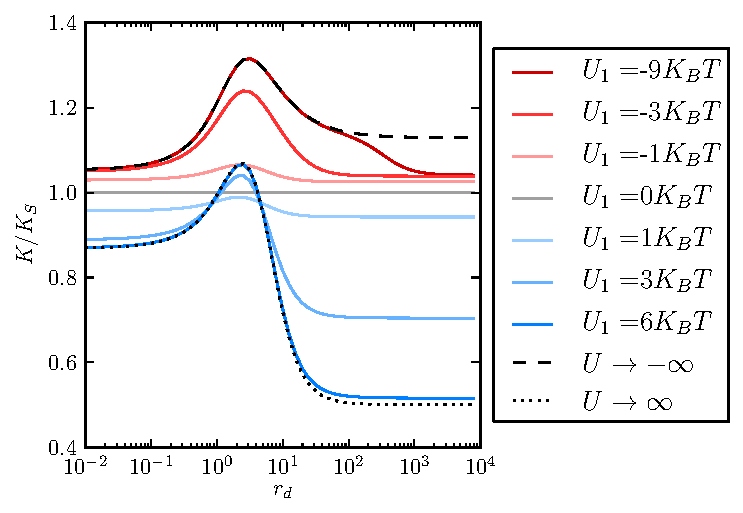
\includegraphics[width = 1 \textwidth]{plots/u1_dependence}
\end{figure}
\end{minipage} \hspace{0.01 \textwidth} \begin{minipage}[t]{.35 \textwidth}
    \begin{figure}[H]
        \caption{Adsorption rate vs decay length for various barrier heights $U_1$. The analytic limits for an infinitely attractive barrier \eqref{attractive_limit} and an infinitely repulsive barrier \eqref{repulsive_limit} are given by dashed and dotted black lines respectively. The barrier spacing in terms of $a$ and $b$ is given in \ref{Parameters}. \label{u1_dependence}}
    \end{figure}
\end{minipage}

Figure \ref{u1_dependence} shows the reaction rate normalized to the Smoluchowski reaction rate $K_S$ as a function of the decay length $r_d$ for different barrier heights $U_1$ as well as the limits for $U_1 \rightarrow -\infty$ of a perfectly attractive barrier and the limit of $U_1 \rightarrow \infty$ of a perfectly repulsive barrier.
It is obvious that for vanishing barrier hight the rate is equal to the ideal Smoluchowski rate \eqref{steady state ideal rate} as one would expect. For an attractive barrier the reaction rate monotonously interpolates between the ideal Smoluchowski rate and the limit of an ideal attractive barrier. For a repulsive barrier the reaction rate monotonously interpolates between the ideal Smoluchowski rate and the limit of an ideal repulsive barrier only for small and large decay lengths. For decay lengths around the resonant decay length the reaction rate first decreases for small $|U_1|$ and then increases to values above the ideal Smoluchowski rate. This is somewhat similar to the dependence of the rate on the barrier spacing observed in \ref{fig:res_l} where for small barrier spacing the resonant reaction rate first decreased below and then increased above the ideal Smoluchowski rate for increasing barrier spacing. \par
One more effect is visible in figure \ref{u1_dependence} that emerges for strongly attractive barriers. The fast switching limit of finitely and infinitely attractive barriers is obviously not equal as the fast switching limit is significantly higher for the infinitely attractive barrier. It is also visible, that for higher $|U_1|$ the reaction rate is similar to the $U_1 \rightarrow -\infty$ limit up to higher decay lengths. To understand this effect reconsider the assumption that has been made in section \ref{lim_long_rd} to derive the slow switching/hight decay length limit of the reaction rate. Here one assumed that for sufficiently slow barrier switching the two states of the barrier can be treated independently. This also implies, that the transient time, that is necessary for the particle density to equilibrate after a barrier switch is small compared to the decay time of the state of the barrier. As it turns out the timescales cannot be separated for diverging $|U_1|$ if the barrier is attractive.\\
The explanation of the effect is most intuitive, if the fluctuations are taken to be a property of the barrier. For an illustration of the density profiles in the slow switching limit for an attractive barrier please refer to figure \ref{asd} A). \\
In its active state the attractive barrier acts as a reservoir that collects particles until the density in the area of the barrier is high enough that the probability of particles to leave the barrier is equal to the probability of particles to enter the barrier. According to the fit conditions derived in \ref{Fit_Conditions} this is given if the quotient of the densities at the sink boundary is equal to the Arrhenius factor $\exp[-U_1/K_B T]$. Also for long times the adsorption rate to the boundary is limited by the ideal Smoluchowski rate to a sink with radius equal to the radius of the outer barrier boundary. Consequently the time for the equilibration of the density profile scales exponentially with the barrier hight and therefore the timescales of density relaxation and barrier fluctuation can not be decoupled, if $U_1$ goes to infinity. For large but finite $U_1$ the reservoir effect of the attractive barrier leads to an increase of the reaction rate even for very slow barrier switching.
\newpage
\section{The one dimensional Limit}
After what has been observed in the previous two sections concerning the influence of barrier spacing and barrier hight, there is one more interesting limit to take which is the limit of $l \rightarrow 0$ i.e. that of an infinitely narrow barrier. This limit is interesting for two reasons. \\
First, it reveals the influence of the barrier curvature. As depicted in figure \ref{fig:llimit_skizze} for very small barrier spacing the system locally looks like a fluctuating barrier in front of an absorbing wall that is supplied with a constant influx of particles from infinity. So, the limit of $l \rightarrow 0$ should show effects that persist even without curvature and in leading order and should give curvature dependent effects in higher orders of $l$.\\
Second, it bridges the gap to the problem of a gated sphere, since for infinitely small barrier spacing and infinite barrier hight the system is equivalent to a sphere, that fluctuates between a state of an absorbing and a state of a reflecting surface.
\\ \vspace{-1 cm}

\begin{minipage}[t]{.372 \textwidth}
    \vspace{0.5 cm}
    \begin{figure}[H]
        \caption{Sketch for the limit of $l\rightarrow 0$. If the spacing of the barrier becomes small relative to the radius of the sink, then also the local curvature of the system vanishes i.e. for a particle that is located in the vicinity of the barrier the system looks like a fluctuating barrier in front of an absorbing wall. Therefore, in this limit the system spatially reduces to one dimension.
    \label{fig:llimit_skizze}}
    \end{figure}
\end{minipage}\hspace{0.04 \textwidth}\begin{minipage}[t]{.608 \textwidth}
    \begin{figure}[H]
        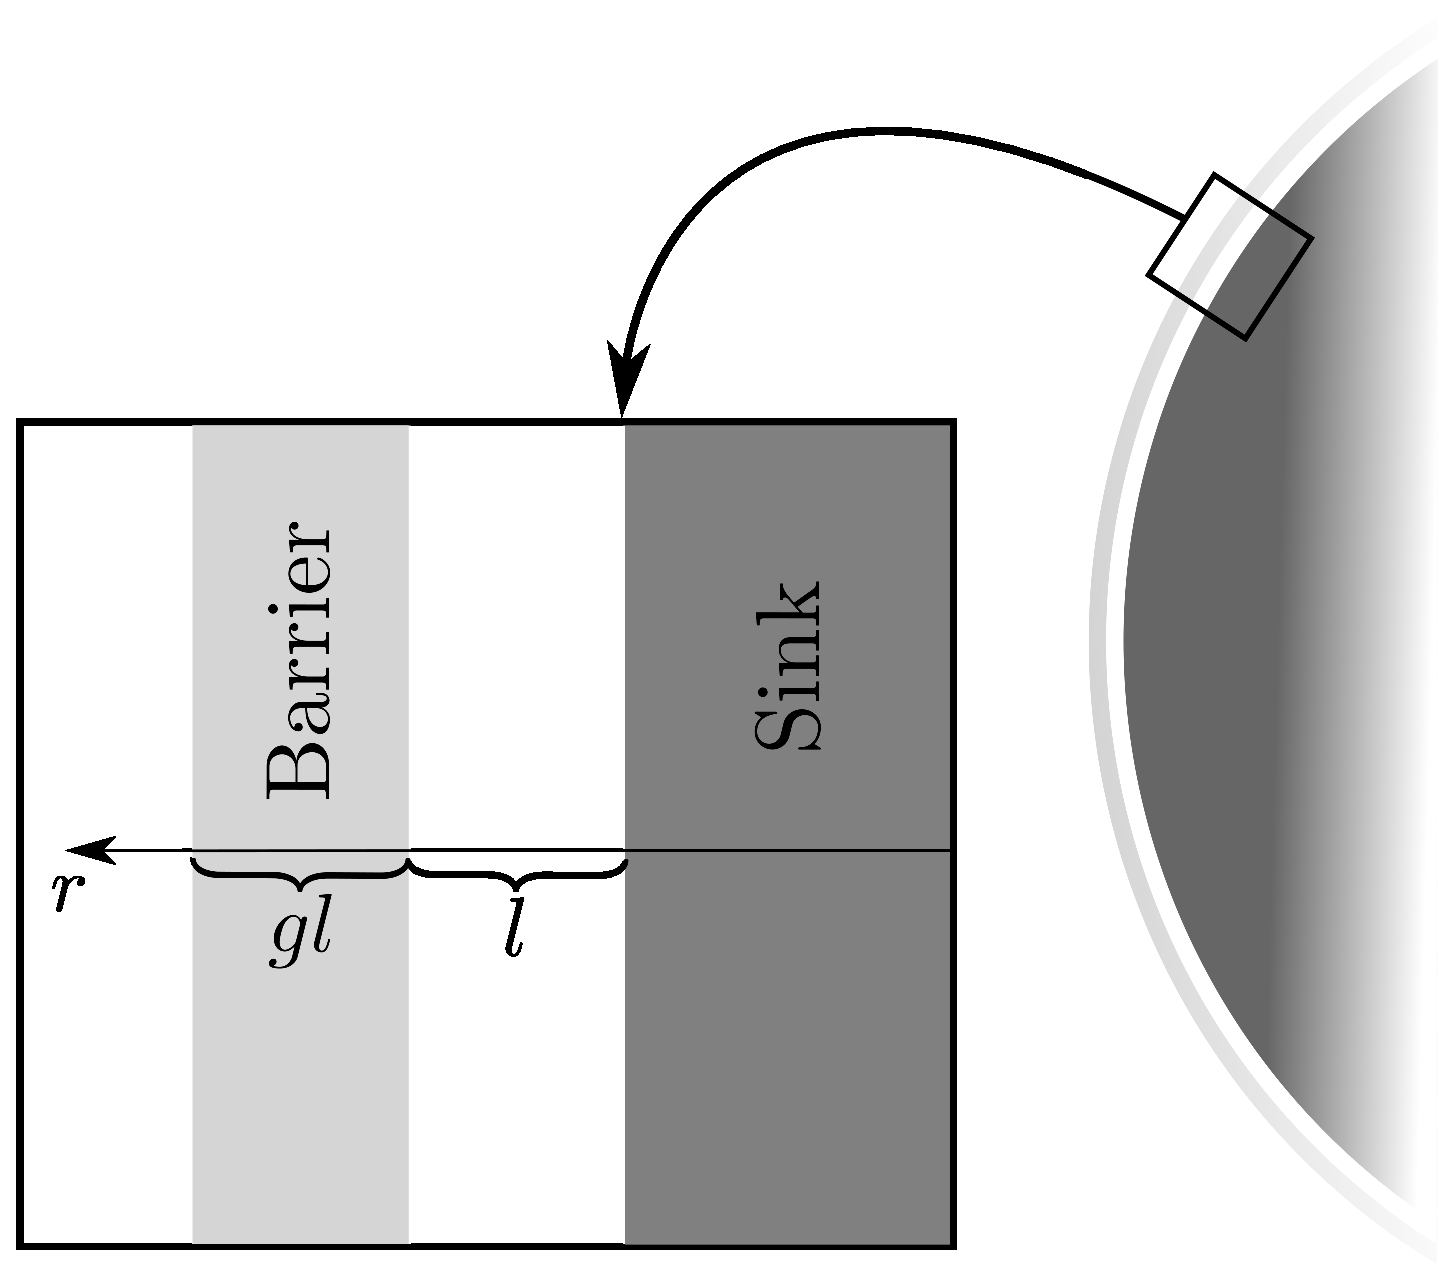
\includegraphics[width = 1 \textwidth]{plots/tlimit.eps}
    \end{figure}
\end{minipage}
\vspace{0.5 cm} \\
The limit is taken for three different situations. For an infinitely attractive barrier, for an infinitely repulsive barrier and for a barrier of finite hight. Therefore the appropriate expressions for the reaction rate \eqref{two_state_rate}, \eqref{attractive_limit} and \eqref{repulsive_limit} are used as a starting point. For each of these expressions one does a Taylor expansion around $l=0$ to obtain the following results:
\begin{itemize}
    \item for a barrier of finite hight:
\end{itemize}
\begin{equation}
    \frac{K}{K_S} \approx 1 + \frac{1}{2}\left(1- \exp\left[\frac{U_1}{K_B T}\right]\right)gl + \mathcal{O}(l^{2}),
    \label{llim_finite}
\end{equation}
\newpage
\begin{itemize}
    \item for an infinitely attractive barrier:
\end{itemize}
\begin{equation}
    \frac{K}{K_S} \approx 1 + \frac{gl}{4} + \mathcal{O}(l^{2}),
    \label{llim_att}
\end{equation}
\begin{itemize}
    \item and for an infinitely repulsive barrier:
\end{itemize}
\begin{equation}
    \frac{K}{K_S} \approx \frac{1+r_d}{1 + 2 r_d} - \frac{(g+1)l}{(2r_d+1)^{2}} + \mathcal{O}(l^{2}).
    \label{llim_rep}
\end{equation}

What is striking is that for the finite and the infinitely attractive barrier the leading order of the reaction rate is simply one. It does nether depend on the barrier hight, nor on the barrier gap to width ratio $g$. And even the fist correction does not depend on the barrier fluctuations. This means, that in the one dimensional limit the fluctuations of the barrier do not have any effect. Consequently, the curvature of the barrier must be crucial for any resonance effects to arise.\\
Concerning the gated sphere one could suspect, that a barrier of finite hight and infinitely small spacing would result in a non ideal sink, i.e. one that does not absorb every particle that comes in contact with its surface since it would have to overcome the barrier first, in which it would succeed only with a probability proportionate to an Arrhenius factor $\exp\left[U_1/K_B T \right]$. As it turns out, this is not the case. To show this, one uses the expression for the Debye reaction rate \eqref{K_Debye} and calculated is for a step shaped potential of hight $U_1$ with boundaries at $1+l$ and $1+l+lg$.
\begin{align}
    K_D   &= 4 \pi D \rho_0 \left\{ \int_{1}^{\infty} \frac{\exp \left[U(r)/K_B T \right]}{r^2} {\rm d} r \right\}^{-1} \nonumber \\
    &=4 \pi D \rho_0 \left\{ \int_{1}^{1+l} \frac{1}{r^2}{\rm d}r + \int_{1+l}^{1+l+lg} \frac{\exp \left[U_1/K_B T \right]}{r^2} {\rm d} r + \int_{1+l+lg}^{\infty}\frac{1}{r^2}{\rm d}r \right\}^{-1} \nonumber \\
    &= 4 \pi D \rho_0 \left\{ \frac{1}{1+l} + \frac{1}{1+l+lg} + \frac{g l}{ (1+l)(1+l+lg)} \right\}^{-1}
    \label{Debye_llimit}
\end{align}
This expression is normalized to the Smoluchowski rate $K_S$ \eqref{steady state ideal rate} and Taylor expanded around $l=0$:
\begin{equation}
    K_D \approx 1+\left(1-\exp\left[\frac{U_1}{K_B T}\right] \right)gl + \mathcal{O}(l^2).
    \label{Debye_taylor}
\end{equation}
It is obvious, that up to linear order in $l$ the small spacing limit of the reaction rate over the fluctuating barrier \eqref{llim_finite} is equal to the average of the Debye rate over the step shaped barrier and the Smoluchowski rate for an ideal barrier. \\
Again, the leading term is equal to one, i.e. for vanishing barrier spacing the barrier has no influence on the adsorption rate. Consequently, the connection to gating can only be made for an infinitely hight fluctuating barrier i.e. in the case when the barrier is assumed to be infinitely hight first before the expansion in $l$ is done (the order of the limit matters, as already noted in section \ref{lim_short_rd}). \\
Indeed, the case of the ideal repulsive barrier \eqref{llim_rep} is the only one, where the reaction rate depends on the barrier fluctuations in the leading order term. The reaction rate interpolated monotonously between $K/K_S = 1$ for $r_d = 0$ and $K/K_S = 0.5$ for $r_d \rightarrow \infty$. These limits are in agreement to what has previously been found for the problem of a gated sphere by Szabo et al. \cite{Szabo1982}. 
They studied the problem of a gated sphere that switches between a first state where its surface reflects incoming particles and a second state where it absorbed incoming particles with a certain surface reaction rate. The called this process opening and closing of the gate.
They found that 
\begin{itemize}
    \item given diffusive relaxation is slow compared to the opening and closing of the gate, the reaction rate is equal to the adsorption rate that would be observed without gating times the probability that the gate is open and
    \item given that the diffusive relaxation is fast compared to the opening and closing of the gate, the spherical sink behaved as if its gate was always open.
\end{itemize}
Since in the case under study the Sink is taken to be ideal, the surface reaction rate of the sink is infinite and the adsorption rate without a barrier is equal to the ideal Smoluchowski rate \eqref{steady state ideal rate}. Also the barrier fluctuations are taken to be symmetric, such that the probability for the barrier to be in one of its two states is equal to one half.
Consequently the findings of Szabo et al. translate to:
\begin{itemize}
    \item slow diffusion relaxation compared to the barrier switching (gating) is equivalent to large $r_d$ where the adsorption rate for the infinitely repulsive barrier of infinitely small spacing is equal to half of the ideal Smoluchowski rate, that would be observed without the barrier,
    \item fast diffusive relaxation and compared to the barrier switching is equivalent to small $r_d$ where the adsorption rate for the infinitely repulsive barrier of infinitely small spacing is equal to the Smoluchowski rate, i.e. it behaves as if the barrier was not there.
\end{itemize}


\newpage
\section{Mapping on a Non-Markovian Description}
\subsection{Common Assumptions}
When an experimentalist would investigate on a realization of the system under study in this thesis he would probably proceed as Shuan Wu et al. \cite{Wu2012a} and do the following: \\ 
He would \emph{first} assume a potential of mean force $U_m(r)$ for the barrier and then calculate the reaction rate using Debye rate theory with a spatially depending diffusivity profile $D(r)$:
\begin{equation}
    K_D^{-1} = \int_{R_s}^{\infty}\frac{\exp[U_m(r)/K_B T]}{4 \pi r^{2} D(r)} {\rm d} r.
    \label{YSDebye}
\end{equation}
and \emph{second}, if the adsorption to the sink in the system would not be ideal but subject to some surface reaction rate $K_S$ he would assume the diffusion controlled and the surface reaction part to independent and calculate the effective reaction rate as:
\begin{equation}
    K_{eff}^{-1} = K_D^{-1} + K_S^{-1}.
    \label{Keff}
\end{equation}
There is a list of problems with these two assumptions that will be outlined in the following discussion. \\
\subsection{First Assumption}
As was shown in section \ref{Numeric_Study} the description of the rate by Debye theory is only valid for smooth potentials and for these only if the switching of the potential is much faster that the diffusion of the Brownian particles. Otherwise both processes couple and the assumption is violated. Moreover, if one sticks to Debye theory and uses the particle density which might be measured and the potential of mean force to calculate an effective spatial diffusivity profile $D_{eff}(r)$ from: 
\begin{equation}
    \rho_D = C \exp\left[\frac{-U_m(r)}{K_B T}\right] \int_{R_s}^{r} \frac{\exp\left[\frac{U_m(r')}{K_B T}\right]}{4 \pi r'^{2} D_{eff}(r)}{\rm d} r'
    \label{Deff}
\end{equation}
this will lead to artificial results. To picture this, one uses two different methods to calculate an effective diffusivity profile. First one uses the Method of Lines as outlined in section \ref{method_of_lines} to derive density profiles for different decay lengths for a smooth potential as given by equation \eqref{generalized_gaussian} and calculates the associated effective diffusivity profile through numeric inversion of equation \eqref{Deff} and second, one sets up Brownian Dynamics simulations as described in section \ref{BDsim}for the same parameters and explicitly tracks the mean square displacement of particles to access the actual diffusivity profile of the system via
\begin{equation}
    \left<\Delta \vec{x}(r)^{2}\right> = 6 D_{eff}(r) \Delta t
    \label{msqd}
\end{equation}
where $\Delta \vec{x}$ is the actual particle displacement and $r$ is its radial position in space.
The results from the first method are given in figure [REF], the results from the second method are given in figure [REF]

\begin{minipage}[t]{.5 \textwidth}
    \begin{figure}[H]
        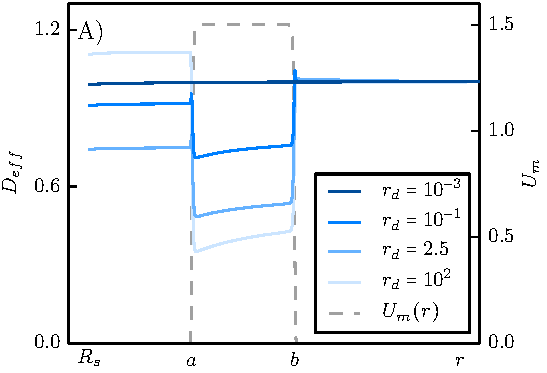
\includegraphics[width = 1 \textwidth]{plots/repulsive_mapping_d.pdf}
    \end{figure}
\end{minipage}\begin{minipage}[t]{.5 \textwidth}
    \begin{figure}[H]
        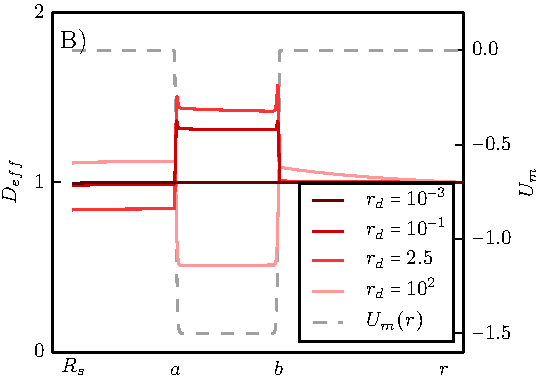
\includegraphics[width = 1 \textwidth]{plots/attractive_mapping_d.pdf}
    \end{figure}
\end{minipage}

\begin{minipage}[t]{1 \textwidth}
    \begin{figure}[H]
        \caption{Effective diffusivity profiles $D_{eff}(r)$ for repulsive (A) and attractive (B) fluctuating barrier for different decay lengths $r_d$ according to Debye rate theory \ref{The_Debye_Reaction_Rate} over a potential of mean force. Results for density profiles calculated by numerical inversion of equation \eqref{Deff}. Necessary density profiles were obtained by the numerical Method of Lines for a smooth potential as given in \eqref{generalized_gaussian} with $U_2$, $a$, and $b$ as given in \eqref{Parameters}.}
    \end{figure}
\end{minipage} \vspace{0.5 cm} \\


\begin{minipage}[t]{.5 \textwidth}
    \begin{figure}[H]
        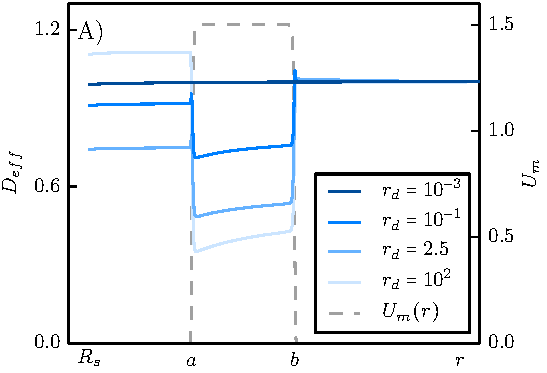
\includegraphics[width = 1 \textwidth]{plots/repulsive_mapping_d.pdf}
    \end{figure}
\end{minipage}\begin{minipage}[t]{.5 \textwidth}
    \begin{figure}[H]
        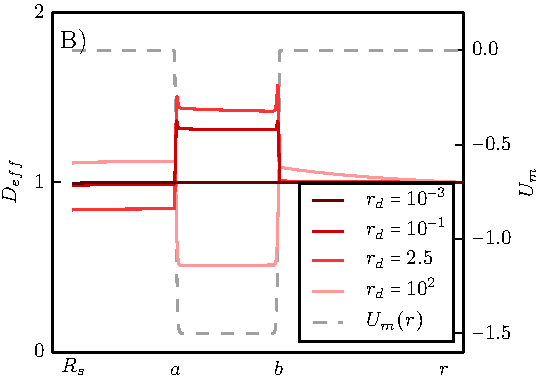
\includegraphics[width = 1 \textwidth]{plots/attractive_mapping_d.pdf}
    \end{figure}
\end{minipage}

\begin{minipage}[t]{1 \textwidth}
    \begin{figure}[H]
        \caption{Effective diffusivity profiles $D_{eff}(r)$ for repulsive (A) and attractive (B) fluctuating barrier for different decay lengths $r_d$ obtained from Brownian Dynamics simulations with a smooth potential as given in \eqref{generalized_gaussian} with $U_2$, $a$, and $b$ as given in \eqref{Parameters}. Spatially resolved mean square displacement was calculated by radial binning of particles positions $\vec{x}$ for each time step, then integrating over $\Delta t$ and separately averaging over the particle square displacement $\Delta \vec{x}^{2}$ for each bin. The effective diffusivity was then calculated by \label{Deff_numeric}}   
    \end{figure}
\end{minipage}



\subsection{Second Assumption}
%This section should bridge the gap from theory to experiments where measurements usually do not give any information of the detailed kinetics of the system but only show fluctuations as a potential of mean force and a spatially depending diffusivity profile.

\section{Summary}
